\documentclass[conference]{IEEEtran}
\IEEEoverridecommandlockouts
\usepackage{cite}
\usepackage{amsmath,amssymb,amsfonts}
\usepackage{graphicx}
\usepackage{textcomp}
\usepackage{xcolor}
\usepackage{booktabs}
\usepackage{multirow}
\usepackage{hyperref}

\begin{document}

\title{A Pre-Registered, Leakage-Free Evaluation of Training-Free Anisotropic-Diffusion Image Fusion: Negative Results on Edge Compensation and Feature Clustering}

\author{\IEEEauthorblockN{M.Tech Research Scholar}
\IEEEauthorblockA{\textit{Department of Computer Science \& Engineering} \\
\textit{Advanced Visual Computing \& Medical Imaging Laboratory} \\
Pre-registration: repository \texttt{Image\_Fusion}, commit \texttt{adae0ed3} (2026-11-24); code commit \texttt{de03fd9}}
}

\maketitle

\begin{abstract}
Multimodal image fusion is routinely evaluated on test sets that overlap the training data of the deep baselines it is compared against, and with metric implementations that are rarely cross-checked. We study a training-free fusion pipeline (ADGF, implemented as \texttt{CADM-MSWN} / frozen \texttt{CADM\_MSWN\_v2}) built from Perona-Malik anisotropic diffusion, a four-component structural decomposition, saliency-based weights regularised by guided filtering, and optional local feature clustering. We pre-registered a selection rule and ran a one-at-a-time ablation of 12 ADGF configurations (covering 15 discrete parameter settings) plus two reference baselines (Averaging and GFF) on 120 development pairs, ranking them by mean rank over five primary metrics ($Q^{AB/F}$, $N^{AB/F}$, $MI$, $SSIM$, $\mathrm{VIFP}$). Two findings were negative relative to our original design. First, additive edge compensation ($\gamma > 0$) degraded results: $N^{AB/F}$ rose from $0.0438$ ($\gamma = 0$) to $0.2888$ ($\gamma = 0.5$) while $Q^{AB/F}$ fell from $0.7187$ to $0.4894$. Second, unclustered global saliency weighting ($K = 1$) ranked first on the development set (mean rank $2.80$ across all 14 configurations, or $2.40$ across 13 excluding GFF; $Q^{AB/F}=0.7107$, $N^{AB/F}=0.0153$, $MI=3.8192$ bits, $SSIM=0.7215$, $\mathrm{VIFP}=0.4764$), ahead of $K = 2$ and $K = 3$. We froze this configuration ($K=1, \gamma=0$) and evaluated the existing benchmark records in \texttt{results/phase4\_test\_metrics.csv} covering 78 held-out test pairs across five datasets---all 15 pairs each from Harvard CT-MRI, PET-MRI, SPECT-MRI, and Lytro ($n=60$ complete pairs), plus 18/42 TNO pairs---against three classical (Averaging, DWT, GFF) and three deep (DenseFuse, U2Fusion, SwinFusion) baselines (with MSRS [361], RoadScene [220], remaining 24 TNO pairs, and ADF, CBF, SWT/NSCT, CDDFuse recorded as pending). Across the 78 evaluated pairs, ADGF loses to GFF on $Q^{AB/F}$ ($0.6758$ vs $0.7394$, Holm $p = 5.35\times 10^{-13}$, Win/Tie/Loss $7/0/71$), $MI$ ($3.9244$ vs $5.2869$ bits, $p = 4.77\times 10^{-9}$, W/T/L $24/0/54$; though ADGF wins on PET-MRI $3.5960$ vs $3.4268$, $p=3.05\times 10^{-4}$), and $\mathrm{VIFP}$ ($0.3987$ vs $0.5007$, $p = 1.25\times 10^{-13}$, W/T/L $1/0/77$), while winning significantly on $SSIM$ ($0.7557$ vs $0.7340$, $p = 9.82\times 10^{-14}$, W/T/L $76/0/2$) and lower $N^{AB/F}$ ($0.0152$ vs $0.0392$, $p = 2.32\times 10^{-12}$, W/T/L $74/0/4$). Against DWT and U2Fusion, ADGF wins significantly on all five primary metrics; against DenseFuse it wins on $Q^{AB/F}$, $MI$, and $\mathrm{VIFP}$; and against SwinFusion it ties on $Q^{AB/F}$ ($0.6758$ vs $0.6675$, Holm $p=0.191$, W/T/L $41/0/37$) and wins on $N^{AB/F}$, $MI$, and $\mathrm{VIFP}$. We also report a provenance audit of baseline training data, metric cross-validation limits, and a correction of an earlier calibration claim.
\end{abstract}

\begin{IEEEkeywords}
image fusion, anisotropic diffusion, guided filtering, pre-registration, evaluation protocol, negative results.
\end{IEEEkeywords}

\section{Introduction}
Multimodal fusion combines complementary sensors into one image: CT and MRI for bone and soft tissue, PET or SPECT with MRI for function and anatomy, infrared with visible for thermal targets and texture, and multi-focus pairs for extended depth of field. Deep methods such as DenseFuse~\cite{li2019densefuse}, U2Fusion~\cite{xu2022u2fusion}, SwinFusion~\cite{ma2022swinfusion}, and CDDFuse~\cite{zhao2023cddfuse} now dominate the literature, but comparisons involving them raise three concerns:
\begin{itemize}
    \item \textbf{Possible train/test overlap.} Several deep baselines were trained on data drawn from the same public sources later used as test sets: U2Fusion~\cite{xu2022u2fusion} trained on RoadScene, Harvard Whole Brain Atlas, and Lytro; SwinFusion~\cite{ma2022swinfusion} trained task-specific weights on MSRS, RoadScene, Harvard CT-MRI/PET-MRI, and Lytro; and CDDFuse~\cite{zhao2023cddfuse} trained on MSRS (whereas DenseFuse~\cite{li2019densefuse} trained exclusively on MS-COCO; Section~\ref{sec:provenance}).
    \item \textbf{Unverified metrics.} Fusion metrics have implementations that differ in padding, normalisation, angle symmetry, and units, so numbers are often not comparable across papers.
    \item \textbf{Cost and interpretability.} Learned models typically require GPUs (or tens of seconds per pair on CPU) and offer no analytic stability guarantees.
\end{itemize}

Training-free methods avoid the first concern by construction. This paper does not claim a new state of the art. Our contributions are: (i) a fully specified training-free diffusion-based pipeline (ADGF) with an explicit numerical stability argument; (ii) a pre-registered selection protocol and a 14-configuration development evaluation on 120 pairs, including two negative findings; (iii) a leakage-controlled benchmark over the 78 held-out test pairs currently recorded in \texttt{results/phase4\_test\_metrics.csv} with paired Wilcoxon tests, Holm correction, effect sizes, and Win/Tie/Loss counts (explicitly flagging pending datasets and baselines); and (iv) an audit of metric implementations and baseline provenance.

\textbf{Relation to prior work.} ADGF is closest to guided-filter fusion (GFF)~\cite{li2013image} and anisotropic-diffusion fusion (ADF)~\cite{bavirisetti2016two}. GFF uses mean filtering for base/detail separation and guided-filtered weight maps; ADF uses diffusion with a different fusion rule. ADGF uses diffusion to define a four-component decomposition and builds weights from local statistics regularised with luminance guidance. Because the final frozen configuration ($K=1, \gamma=0$) is structurally near GFF, we treat GFF as the primary comparator and claim no algorithmic novelty beyond this combination and the evaluation findings.

\section{Method}
All operations run on normalised luminance in $[0, 1]$.

\subsection{Colour handling}
Sources are converted to ITU-R BT.601 YCbCr:
\begin{align}
Y &= 0.299R + 0.587G + 0.114B, \\
Cb &= -0.168736R - 0.331264G + 0.5B + 0.5, \\
Cr &= 0.5R - 0.418688G - 0.081312B + 0.5.
\end{align}
For MRI with PET or SPECT, chrominance is taken from the functional image; for two colour inputs it is averaged. The fused RGB image is obtained by the inverse transform and clipped to $[0, 1]$.

\subsection{Anisotropic diffusion}
We use Perona-Malik diffusion~\cite{perona1990scale}: $\partial u / \partial t = \mathrm{div}(g(|\nabla u|)\nabla u)$, $u(0) = Y$, $g(s) = \exp(-(s/\kappa)^2)$, $\kappa = 30/255 \approx 0.1176$. The explicit 4-neighbour scheme is:
\begin{equation}
u^{t+1} = u^t + \lambda \sum_{d \in \{N,S,E,W\}} g(\nabla_d u^t)\nabla_d u^t.
\end{equation}
\textbf{Stability.} Because $0 < g \le 1$, the explicit 4-neighbour update is a convex-type averaging step when $\lambda \le 1/4$, giving a maximum-principle (non-divergence) guarantee. We use $\lambda = 0.20$ and $T = 20$ iterations. This is a statement about the numerical scheme, not about fusion quality.

\subsection{Four-component decomposition}
With $GT = u(T)$ (gross texture): gross edge $GE = |\nabla GT|$; fine texture $FT = Y - GT$; fine edge $FE = \max(0, |\nabla Y| - GE)$. When $\gamma = 0$, $Y = GT + FT$ holds identically.

\subsection{Weighted fusion}
For each source and pixel $x$, local statistics over a $7 \times 7$ box window (\texttt{BORDER\_REFLECT}) yield component saliency maps from local energy, variance, and spatial frequency. Weights are normalised across sources and refined by guided filtering~\cite{he2013guided} with luminance guidance (radius $r = 5$, $\epsilon = 10^{-4}$) followed by re-normalisation. When $K > 1$, pixels are first clustered per source on the local $[\mu_w, \sigma_w^2, SF_w]$ vector and weights are computed per cluster; $K = 1$ uses one global saliency weighting. The fused luminance is:
\begin{equation}
Y_{\text{fused}} = \alpha\, GT' + \beta\, FT' + \gamma\, \mathrm{sign}(FT')(GE' + FE'),
\end{equation}
where primes denote weight-fused components, $\alpha = \beta = 1$, and $\gamma$ controls edge compensation.

\textbf{Terminology.} The method is \emph{training-free} with no learned weights. It does have fixed hyperparameters ($\kappa=0.1176$, $\lambda=0.20$, $T=20$, $w=7$, $r=5$, $\epsilon=10^{-4}$, $K=1$, $\alpha=\beta=1$, $\gamma=0$), fixed by the pre-registered rule, so we do not say ``zero parameters''.

\section{Evaluation Protocol and Audit}

\subsection{Correction of an earlier claim}
An earlier internal draft stated that no test images were used for calibration. That was inaccurate: exploratory checks inspected \texttt{pair1\_mri\_ct} (\texttt{CT-MRI\_16003}) and \texttt{pair4\_multifocus} (\texttt{lytro\_01}). All five sanity pairs are therefore classed as development data and excluded from all test statistics.

\subsection{Data splits and verification}
Table~\ref{tab:splits} summarises the splits in \texttt{splits.yaml}.
\begin{table}[htbp]
\caption{Pre-Registered Development and Held-Out Test Splits.}
\label{tab:splits}
\centering
\begin{tabular}{lp{4.8cm}r}
\toprule
\textbf{Split} & \textbf{Composition} & \textbf{Pairs} \\
\midrule
Development & MSRS 100 (\texttt{train}); Harvard CT-MRI 5, PET-MRI 5, SPECT-MRI 5; Lytro 5 & 120 \\
Test & Harvard CT-MRI 15, PET-MRI 15, SPECT-MRI 15; Lytro 15; MSRS 361; RoadScene 220; TNO 42 & 683 \\
\bottomrule
\end{tabular}
\end{table}

\textbf{Verification:} (a) \emph{Reconciling 704 vs 683:} The verified dataset inventory (\texttt{all\_datasets\_verified\_inventory.json}) catalogs 704 pairs across the seven evaluation sources (20 each for Harvard CT/PET/SPECT-MRI and Lytro, 221 for RoadScene, 361 for MSRS test, 42 for TNO). Moving 5 pairs each from the four 20-pair sets into development ($20$ pairs) and excluding \texttt{roadscene\_FLIR\_00006} (1 exploratory sanity pair) removes $21$ pairs, leaving $704 - 21 = 683$ test pairs. (b) \emph{Disjointness:} A SHA256 and ID audit of \texttt{splits.yaml} confirmed zero overlapping IDs, paths, or source-image SHA256 hashes between the 120 dev pairs and 683 test pairs. (c) \emph{Sanity pairs:} By SHA256 matching, \texttt{pair1\_mri\_ct} (\texttt{CT-MRI\_16003}), \texttt{pair2\_mri\_pet} (\texttt{PET-MRI\_25015}), \texttt{pair4\_multifocus} (\texttt{lytro\_01}), and \texttt{pair5\_mri\_spect} (\texttt{SPECT-MRI\_10007}) sit inside the 120 dev pairs, while \texttt{pair3\_ir\_vis} (\texttt{FLIR\_00006}) is excluded from both splits.

\subsection{Metrics and cross-validation}
Primary metrics: $Q^{AB/F}$ ($\uparrow$)~\cite{xydeas2000objective,petrovic2005}, $N^{AB/F}$ ($\downarrow$)~\cite{petrovic2005}, $MI$ ($\uparrow$), $SSIM$ ($\uparrow$)~\cite{wang2004image}, and $\mathrm{VIFP}$ ($\uparrow$)~\cite{sheikh2006image}. Secondary, descriptive only: $EN$, $SD$, $SF$, $AG$. Our $MI$ implementation (\texttt{metrics/information.py}) uses $\log_2$ on 256-bin joint histograms and \textbf{sums} $MI(F,I_1)+MI(F,I_2)$ in \textbf{bits} (when comparing against \texttt{sklearn.metrics.mutual\_info\_score}, which returns nats, \texttt{cross\_validate\_metrics\_external.py} divides by $\ln 2$, matching with $|\Delta|=0.0000$).

Table~\ref{tab:metrics_cv} summarises metric cross-validation. \texttt{compute\_ssim} wraps \texttt{skimage.metrics.structural\_similarity} (\texttt{data\_range=1.0}) and \texttt{compute\_vif} wraps \texttt{sewar.full\_ref.vifp} ($\sigma_{nsq}^2=2.0$), so $|\Delta|=0.0000$ confirms wiring rather than independent validation. \texttt{sewar} SSIM differs by $0.0529$--$0.3439$ on $[0,255]$ luminance ($0.0019$--$0.0427$ in an earlier unscaled run) due to valid convolution vs \texttt{skimage} reflection padding; we use \texttt{skimage}. For $Q^{AB/F}$, we compared against the external CDDFuse \texttt{Evaluator.Qabf} across 15 deep-baseline outputs ($|\Delta|=0.0113$--$0.0395$, $77.61\%$--$97.95\%$ agreement); for $N^{AB/F}$, no external Python reference was available beyond our internal re-implementation ($|\Delta|=0.0000$).

\begin{table}[htbp]
\caption{Metric Wrapper Provenance and Cross-Validation Summary.}
\label{tab:metrics_cv}
\centering
\begin{tabular}{llcc}
\toprule
\textbf{Metric} & \textbf{Comparator} & \textbf{Direct Wrap?} & \textbf{Observed $|\Delta|$} \\
\midrule
$SSIM$ & \texttt{skimage} (reflect) & Yes & $0.0000$ \\
$SSIM$ & \texttt{sewar} (valid, no pad) & No & $0.0529$--$0.3439$ \\
$\mathrm{VIFP}$ & \texttt{sewar.full\_ref.vifp} & Yes & $0.0000$ \\
$MI$ [bits] & \texttt{sklearn} $/ \ln 2$ & No & $0.0000$ \\
$Q^{AB/F}$ & CDDFuse \texttt{Evaluator} & No & $0.0113$--$0.0395$ \\
$N^{AB/F}$ & Internal Petrovic ref. & No & $0.0000$ \\
\bottomrule
\end{tabular}
\end{table}

\subsection{Baseline training provenance}
\label{sec:provenance}
Table~\ref{tab:provenance} audits each deep baseline from its paper and released repository code. Flagged baselines are retained rather than excluded. FusionGAN~\cite{ma2019fusiongan}, DDFM~\cite{zhao2023ddfm}, and PIAFusion~\cite{tang2022piafusion} are documented as blocked in \texttt{BLOCKERS.md} and \texttt{deep\_baselines\_smoke\_test.json}.

\begin{table*}[htbp]
\caption{Deep Baseline Training Data Provenance and Test-Set Overlap Audit.}
\label{tab:provenance}
\centering
\begin{tabular}{lllp{4.8cm}l}
\toprule
\textbf{Baseline} & \textbf{Reported Training Data} & \textbf{Weights Used} & \textbf{Overlap with Our Test Sets} & \textbf{Source} \\
\midrule
DenseFuse~\cite{li2019densefuse} & MS-COCO (80k natural images) & Yes (\texttt{densefuse\_weights.pkl}) & None (zero multimodal test overlap) & Li \& Wu~\cite{li2019densefuse}; \texttt{densefuse.py} \\
U2Fusion~\cite{xu2022u2fusion} & RoadScene, Harvard Atlas, Lytro & Yes (\texttt{u2fusion\_model.pth}) & \textbf{High (flagged):} RoadScene, Harvard, Lytro & Xu et al.~\cite{xu2022u2fusion}; \texttt{u2fusion.py} \\
SwinFusion~\cite{ma2022swinfusion} & MSRS, RoadScene, Harvard, Lytro & Yes (\texttt{ivif/ct\_mri/mff\_10000\_E.pth}) & \textbf{High (flagged):} MSRS, RoadScene, Harvard, Lytro & Ma et al.~\cite{ma2022swinfusion}; \texttt{swinfusion.py} \\
CDDFuse~\cite{zhao2023cddfuse} & MSRS (IVF), Harvard (MIF) & Smoke-tested; pending Phase 4 CSV & \textbf{High (flagged):} MSRS, Harvard & Zhao et al.~\cite{zhao2023cddfuse}; \texttt{cddfuse.py} \\
\bottomrule
\end{tabular}
\end{table*}

\subsection{Pre-registered selection rule}
Configurations were varied one parameter at a time from a reference anchor ($\gamma=0.0$, linear, $r=5$, $T=20$, $K=3$) and ranked by mean rank over the five primary metrics on the 120 dev pairs. Quoted verbatim from \texttt{selection\_rule.md}: \emph{``If two or more configurations achieve an identical Mean Rank $\bar{R}(c)$, ties are broken deterministically by lowest mean inference latency on the 120 dev pairs: $c_{\text{tie-winner}} = \arg\min_{c \in \text{Ties}} \text{Mean Latency}(c)$.''} Under Section 1.4 of \texttt{selection\_rule.md}, the prototype is retained if no candidate achieves strictly lower mean rank.

\section{Development-Set Ablation (120 pairs)}
Reconciling the 15 discrete parameter settings, 12 OAT ADGF runs (\texttt{selection\_rule.md}), 13-row draft table, and 14-row CSV (\texttt{dev\_ablation\_ranked.csv}): four dimensions share the anchor \texttt{gamma\_0.0\_no\_edge\_comp} ($T=20, K=3, \gamma=0, r=5$, linear), yielding 12 ADGF runs plus 2 reference baselines (\texttt{Averaging} and \texttt{GFF}) = 14 configurations in \texttt{dev\_ablation\_ranked.csv} (the earlier 13-row draft omitted GFF, shifting $K=1$'s mean rank from $2.80$ to $2.40$). The winning $K=1$ configuration uses $T=20, \kappa=0.1176, \lambda=0.20, w=7, r=5, \epsilon=10^{-4}$, linear normalisation, $\alpha=\beta=1.0, \gamma=0.0$. Note that $K=3$ was run as the \texttt{gamma\_0.0\_no\_edge\_comp} anchor (Rank 6/14).

\begin{table*}[htbp]
\caption{Pre-Registered Development-Set Ranking (120 Pairs, 5 Primary Metrics, 14 Configurations from \texttt{dev\_ablation\_ranked.csv}).}
\label{tab:dev_ablation}
\centering
\begin{tabular}{rlccccccc}
\toprule
\textbf{Rank} & \textbf{Configuration} & \textbf{Mean Rank (14 / 13)} & $Q^{AB/F}$ ($\uparrow$) & $N^{AB/F}$ ($\downarrow$) & $MI$ [bits] ($\uparrow$) & $SSIM$ ($\uparrow$) & $\mathrm{VIFP}$ ($\uparrow$) & \textbf{Lat (ms)} \\
\midrule
\textbf{1} & \textbf{\texttt{K = 1} (no clustering; frozen)} & \textbf{2.80 (2.40)} & \textbf{0.7107} & \textbf{0.0153} & \textbf{3.8192} & \textbf{0.7215} & \textbf{0.4764} & \textbf{3062.7} \\
2 & GFF (reference) & 3.40 (---) & 0.7356 & 0.0630 & 3.4553 & 0.7016 & 0.5034 & 2273.4 \\
3 & \texttt{K = 2} & 5.20 (4.20) & 0.6410 & 0.0966 & 3.2335 & 0.6627 & 0.3965 & 12654.8 \\
4 & Averaging (reference) & 6.20 (5.60) & 0.4128 & 0.0000 & 2.9637 & 0.7287 & 0.3570 & 409.5 \\
5 & \texttt{softmax tau = 1.0} & 6.60 (6.00) & 0.4727 & 0.0052 & 2.9344 & 0.7309 & 0.3542 & 2239.3 \\
6 & \texttt{gamma = 0.0} (anchor, $K=3$) & 6.60 (5.80) & 0.7187 & 0.0438 & 2.9492 & 0.6381 & 0.3679 & 3413.2 \\
7 & \texttt{softmax tau = 0.5} & 7.20 (6.60) & 0.4918 & 0.0140 & 2.9329 & 0.7288 & 0.3478 & 2411.1 \\
8 & \texttt{T = 5} & 7.60 (6.60) & 0.6096 & 0.1302 & 2.9861 & 0.6389 & 0.3680 & 4548.1 \\
9 & \texttt{T = 10} & 7.60 (6.60) & 0.6114 & 0.1296 & 2.9665 & 0.6385 & 0.3680 & 6834.8 \\
10 & \texttt{softmax tau = 0.1} & 7.80 (7.20) & 0.6215 & 0.0160 & 2.9138 & 0.7128 & 0.3309 & 1678.0 \\
11 & \texttt{guided radius 9} & 9.40 (8.40) & 0.6022 & 0.1213 & 2.8325 & 0.6399 & 0.3553 & 2175.0 \\
12 & \texttt{guided radius 13} & 9.80 (8.80) & 0.5967 & 0.1155 & 2.7663 & 0.6420 & 0.3499 & 2837.1 \\
13 & \texttt{gamma = 0.25} & 11.00 (10.00) & 0.6459 & 0.1327 & 2.5118 & 0.6033 & 0.3324 & 1613.2 \\
14 & \texttt{Prototype (gamma = 0.5)} & 13.60 (12.60) & 0.4894 & 0.2888 & 2.1403 & 0.5444 & 0.2875 & 4686.0 \\
\bottomrule
\end{tabular}
\end{table*}

\subsection{Edge compensation ($\gamma > 0$) hurt in our implementation}
The prototype used $\gamma = 0.5$ and ranked last. Moving to $\gamma = 0$ reduced $N^{AB/F}$ from $0.2888$ to $0.0438$ (about $85\%$) and raised $Q^{AB/F}$ from $0.4894$ to $0.7187$. Because $GE$ and $FE$ are non-negative gradient magnitudes, adding them introduces positive bias and sign-ambiguous structure instead of restoring edges. Signed detail injection is untested here; we report a negative result for additive unsigned gradient injection only.

\subsection{Clustering did not help}
$K = 1$ outperformed $K = 2$ and $K = 3$ on all primary metrics except $Q^{AB/F}$ ($K=3$: $0.7187$ vs $0.7107$, at nearly $3\times$ the noise $0.0438$ vs $0.0153$) and was roughly $4\times$ faster than $K=2$ ($3.06\text{ s}$ vs $12.65\text{ s}$). Discrete cluster masks introducing seams that guided filtering only partly removes is an untested hypothesis.

\subsection{Caveats}
$K = 1$ is best by mean rank, not on every metric: Averaging ($0.7287$) and $\tau=1.0$ ($0.7309$) have higher $SSIM$, GFF has higher $Q^{AB/F}$ ($0.7356$) and $\mathrm{VIFP}$ ($0.5034$), and $\gamma=0$ ($K=3$) has slightly higher $Q^{AB/F}$ ($0.7187$). Because the OAT sweep ignores interactions and ranking/reporting share the 120 dev pairs, Table~\ref{tab:dev_ablation} values are in-sample.

\section{Results}

\subsection{Development illustration (5 sanity pairs)}
Table~\ref{tab:sanity5} reproduces the five development sanity pairs alongside the frozen ADGF ($K=1, \gamma=0$) configuration.
\begin{table}[htbp]
\caption{Primary Metrics on the Five Development Sanity Pairs.}
\label{tab:sanity5}
\centering
\scriptsize
\begin{tabular}{llccccc}
\toprule
\textbf{Pair} & \textbf{Method} & $Q^{AB/F}$ & $N^{AB/F}$ & $MI$ & $SSIM$ & $\mathrm{VIFP}$ \\
\midrule
\multirow{7}{*}{pair1 (CT-MRI)}
& Averaging & 0.3695 & 0.0000 & 3.6736 & 0.6705 & 0.2756 \\
& DWT & 0.5624 & 0.0714 & 1.9886 & 0.6627 & 0.1952 \\
& GFF & 0.6856 & 0.0224 & 2.1476 & 0.6945 & 0.3992 \\
& ADGF proto & 0.3938 & 0.2688 & 1.9128 & 0.6441 & 0.1683 \\
& \textbf{ADGF frozen} & \textbf{0.6793} & \textbf{0.0184} & \textbf{2.5720} & \textbf{0.7179} & \textbf{0.3599} \\
& DenseFuse & 0.6037 & 0.0531 & 2.6915 & 0.3022 & 0.2966 \\
& SwinFusion & 0.7117 & 0.0424 & 2.5837 & 0.7267 & 0.3660 \\
\midrule
\multirow{5}{*}{pair2 (PET-MRI)}
& GFF & 0.8361 & 0.0269 & 2.9726 & 0.7897 & 0.5047 \\
& ADGF proto & 0.4688 & 0.2923 & 2.1486 & 0.7393 & 0.2265 \\
& \textbf{ADGF frozen} & \textbf{0.8097} & \textbf{0.0062} & \textbf{3.2241} & \textbf{0.7939} & \textbf{0.4933} \\
& DenseFuse & 0.7170 & 0.0413 & 2.8471 & 0.2818 & 0.3791 \\
& SwinFusion & 0.8377 & 0.0331 & 2.7916 & 0.2615 & 0.4587 \\
\midrule
\multirow{4}{*}{pair3 (RoadScene)}
& GFF & 0.7124 & 0.0716 & 4.1860 & 0.6355 & 0.4363 \\
& ADGF proto & 0.2929 & 0.3684 & 1.9648 & 0.4625 & 0.1275 \\
& \textbf{ADGF frozen} & \textbf{0.5355} & \textbf{0.0254} & \textbf{3.2059} & \textbf{0.6694} & \textbf{0.2802} \\
& SwinFusion & 0.4348 & 0.0496 & 3.1877 & 0.6796 & 0.3313 \\
\midrule
\multirow{4}{*}{pair4 (Lytro)}
& GFF & 0.7604 & 0.0659 & 6.6628 & 0.8682 & 0.7196 \\
& ADGF proto & 0.1831 & 0.2241 & 2.7561 & 0.6130 & 0.1767 \\
& \textbf{ADGF frozen} & \textbf{0.7314} & \textbf{0.0038} & \textbf{6.0279} & \textbf{0.8906} & \textbf{0.6273} \\
& SwinFusion & 0.7341 & 0.0192 & 5.7291 & 0.9045 & 0.6255 \\
\midrule
\multirow{4}{*}{pair5 (SPECT-MRI)}
& GFF & 0.8209 & 0.0361 & 3.7563 & 0.6899 & 0.5034 \\
& ADGF proto & 0.3994 & 0.4715 & 2.1754 & 0.5744 & 0.2842 \\
& \textbf{ADGF frozen} & \textbf{0.8066} & \textbf{0.0147} & \textbf{3.7174} & \textbf{0.6984} & \textbf{0.5197} \\
& SwinFusion & 0.8187 & 0.0431 & 3.0364 & 0.3474 & 0.4522 \\
\bottomrule
\end{tabular}
\end{table}

\subsection{Held-out test results (\texttt{results/phase4\_test\_metrics.csv})}
Table~\ref{tab:test_results} reports Mean $\pm$ Std across the 78 held-out test pairs currently recorded in \texttt{results/phase4\_test\_metrics.csv} (complete $n=15$ for CT-MRI, PET-MRI, SPECT-MRI, Lytro; partial $n=18/42$ for TNO). MSRS (361), RoadScene (220), the remaining 24 TNO pairs, and baselines ADF, CBF, SWT/NSCT, and CDDFuse remain unrun in \texttt{phase4\_test\_metrics.csv}. Table~\ref{tab:wilcoxon} reports paired Wilcoxon signed-rank tests, Holm-Bonferroni adjusted $p$-values, effect sizes $r=|Z|/\sqrt{N}$, and Win/Tie/Loss counts.

\begin{table*}[htbp]
\caption{Held-Out Test Results from \texttt{results/phase4\_test\_metrics.csv} (Mean $\pm$ Std). Starred (*) Baselines Have Training-Domain Overlap.}
\label{tab:test_results}
\centering
\scriptsize
\begin{tabular}{llccccc}
\toprule
\textbf{Dataset ($n$)} & \textbf{Method} & $Q^{AB/F}$ ($\uparrow$) & $N^{AB/F}$ ($\downarrow$) & $MI$ [bits] ($\uparrow$) & $SSIM$ ($\uparrow$) & $\mathrm{VIFP}$ ($\uparrow$) \\
\midrule
\multirow{7}{*}{CT-MRI (15/15)}
& Averaging & 0.3949$\pm$0.0202 & 0.0000$\pm$0.0000 & 3.7067$\pm$0.2242 & 0.7599$\pm$0.0497 & 0.2419$\pm$0.0259 \\
& DWT & 0.5479$\pm$0.0245 & 0.0732$\pm$0.0067 & 2.4466$\pm$0.2711 & 0.7364$\pm$0.0474 & 0.1892$\pm$0.0221 \\
& GFF & 0.6453$\pm$0.0276 & 0.0317$\pm$0.0082 & 2.9677$\pm$0.6141 & 0.7491$\pm$0.0412 & 0.3621$\pm$0.0273 \\
& DenseFuse & 0.5074$\pm$0.0429 & 0.0064$\pm$0.0013 & 2.9534$\pm$0.2259 & 0.7665$\pm$0.0451 & 0.2824$\pm$0.0221 \\
& U2Fusion* & 0.3927$\pm$0.0135 & 0.0213$\pm$0.0057 & 2.7362$\pm$0.2814 & 0.7530$\pm$0.0496 & 0.2218$\pm$0.0219 \\
& SwinFusion* & 0.6167$\pm$0.0310 & 0.0416$\pm$0.0072 & 2.9269$\pm$0.3011 & 0.7786$\pm$0.0402 & 0.2958$\pm$0.0264 \\
& \textbf{ADGF ($K=1,\gamma=0$)} & 0.6296$\pm$0.0185 & 0.0171$\pm$0.0026 & 2.9380$\pm$0.2692 & 0.7675$\pm$0.0408 & 0.3049$\pm$0.0234 \\
\midrule
\multirow{7}{*}{PET-MRI (15/15)}
& Averaging & 0.4453$\pm$0.0139 & 0.0003$\pm$0.0001 & 4.1103$\pm$0.1589 & 0.7042$\pm$0.0167 & 0.3708$\pm$0.0207 \\
& DWT & 0.5976$\pm$0.0153 & 0.0539$\pm$0.0055 & 2.3998$\pm$0.0915 & 0.7043$\pm$0.0166 & 0.2463$\pm$0.0142 \\
& GFF & 0.7952$\pm$0.0220 & 0.0149$\pm$0.0012 & 3.4268$\pm$0.0951 & 0.7410$\pm$0.0195 & 0.4487$\pm$0.0235 \\
& DenseFuse & 0.6475$\pm$0.0262 & 0.0044$\pm$0.0001 & 3.0014$\pm$0.1040 & 0.7427$\pm$0.0194 & 0.3304$\pm$0.0202 \\
& U2Fusion* & 0.5134$\pm$0.0118 & 0.0291$\pm$0.0011 & 2.5814$\pm$0.1196 & 0.7095$\pm$0.0193 & 0.2373$\pm$0.0119 \\
& SwinFusion* & 0.7424$\pm$0.0225 & 0.0393$\pm$0.0039 & 3.1397$\pm$0.1081 & 0.7528$\pm$0.0166 & 0.3669$\pm$0.0214 \\
& \textbf{ADGF ($K=1,\gamma=0$)} & 0.7277$\pm$0.0305 & 0.0051$\pm$0.0003 & 3.5960$\pm$0.0915 & 0.7502$\pm$0.0180 & 0.4101$\pm$0.0270 \\
\midrule
\multirow{7}{*}{SPECT-MRI (15/15)}
& Averaging & 0.3988$\pm$0.0116 & 0.0000$\pm$0.0000 & 4.1074$\pm$0.0608 & 0.6999$\pm$0.0104 & 0.2584$\pm$0.0242 \\
& DWT & 0.5725$\pm$0.0172 & 0.0959$\pm$0.0047 & 2.7708$\pm$0.1038 & 0.6788$\pm$0.0110 & 0.2223$\pm$0.0162 \\
& GFF & 0.7775$\pm$0.0155 & 0.0478$\pm$0.0030 & 5.4735$\pm$0.2312 & 0.6701$\pm$0.0129 & 0.4938$\pm$0.0042 \\
& DenseFuse & 0.4516$\pm$0.0220 & 0.0028$\pm$0.0007 & 3.4438$\pm$0.1206 & 0.7009$\pm$0.0108 & 0.2709$\pm$0.0193 \\
& U2Fusion* & 0.4675$\pm$0.0127 & 0.0344$\pm$0.0075 & 3.0970$\pm$0.1267 & 0.6831$\pm$0.0112 & 0.2356$\pm$0.0141 \\
& SwinFusion* & 0.6351$\pm$0.0197 & 0.0362$\pm$0.0058 & 3.2738$\pm$0.1375 & 0.7019$\pm$0.0123 & 0.2784$\pm$0.0179 \\
& \textbf{ADGF ($K=1,\gamma=0$)} & 0.7001$\pm$0.0246 & 0.0257$\pm$0.0039 & 3.5743$\pm$0.1046 & 0.6901$\pm$0.0129 & 0.3314$\pm$0.0236 \\
\midrule
\multirow{7}{*}{Lytro (15/15)}
& Averaging & 0.5936$\pm$0.0922 & 0.0000$\pm$0.0000 & 6.4434$\pm$1.2809 & 0.8794$\pm$0.0651 & 0.5412$\pm$0.0935 \\
& DWT & 0.6808$\pm$0.0511 & 0.0691$\pm$0.0063 & 6.2378$\pm$1.2410 & 0.8381$\pm$0.0717 & 0.5182$\pm$0.0992 \\
& GFF & 0.7763$\pm$0.0324 & 0.0648$\pm$0.0116 & 8.4813$\pm$0.9150 & 0.8349$\pm$0.0716 & 0.6908$\pm$0.0463 \\
& DenseFuse & 0.4919$\pm$0.1231 & 0.0011$\pm$0.0005 & 6.4107$\pm$1.2592 & 0.8776$\pm$0.0647 & 0.5192$\pm$0.0948 \\
& U2Fusion* & 0.5348$\pm$0.0890 & 0.0355$\pm$0.0101 & 6.1805$\pm$1.1604 & 0.8539$\pm$0.0634 & 0.5021$\pm$0.0932 \\
& SwinFusion* & 0.7462$\pm$0.0388 & 0.0189$\pm$0.0040 & 6.5426$\pm$1.1040 & 0.8625$\pm$0.0691 & 0.5827$\pm$0.0740 \\
& \textbf{ADGF ($K=1,\gamma=0$)} & 0.7246$\pm$0.0511 & 0.0110$\pm$0.0079 & 6.5721$\pm$1.3137 & 0.8529$\pm$0.0729 & 0.5745$\pm$0.0926 \\
\midrule
\multirow{7}{*}{TNO (18/42 partial)}
& Averaging & 0.3975$\pm$0.0995 & 0.0000$\pm$0.0000 & 2.5539$\pm$0.9439 & 0.7589$\pm$0.1048 & 0.3188$\pm$0.1148 \\
& DWT & 0.5327$\pm$0.0942 & 0.1147$\pm$0.0380 & 2.1177$\pm$0.8929 & 0.7207$\pm$0.1110 & 0.2867$\pm$0.1168 \\
& GFF & 0.7091$\pm$0.0663 & 0.0371$\pm$0.0252 & 5.9523$\pm$1.3736 & 0.6845$\pm$0.1050 & 0.5066$\pm$0.0525 \\
& DenseFuse & 0.3930$\pm$0.1113 & 0.0019$\pm$0.0010 & 3.0226$\pm$0.7917 & 0.7449$\pm$0.1063 & 0.3322$\pm$0.1023 \\
& U2Fusion & 0.3692$\pm$0.1049 & 0.0398$\pm$0.0226 & 2.7417$\pm$0.7809 & 0.7079$\pm$0.1144 & 0.2824$\pm$0.1222 \\
& SwinFusion & 0.6089$\pm$0.0797 & 0.1244$\pm$0.0447 & 3.2230$\pm$0.7934 & 0.7071$\pm$0.0987 & 0.3910$\pm$0.1054 \\
& \textbf{ADGF ($K=1,\gamma=0$)} & 0.6101$\pm$0.0937 & 0.0168$\pm$0.0145 & 3.1052$\pm$0.7065 & 0.7243$\pm$0.1130 & 0.3769$\pm$0.1005 \\
\midrule
\multirow{7}{*}{Pooled Complete (60)}
& Averaging & 0.4581$\pm$0.0939 & 0.0001$\pm$0.0001 & 4.5919$\pm$1.2639 & 0.7609$\pm$0.0838 & 0.3531$\pm$0.1303 \\
& DWT & 0.5997$\pm$0.0586 & 0.0730$\pm$0.0162 & 3.4637$\pm$1.7369 & 0.7394$\pm$0.0747 & 0.2940$\pm$0.1415 \\
& GFF & 0.7486$\pm$0.0654 & 0.0398$\pm$0.0200 & 5.0873$\pm$2.2612 & 0.7488$\pm$0.0723 & 0.4989$\pm$0.1248 \\
& DenseFuse & 0.5246$\pm$0.0993 & 0.0037$\pm$0.0021 & 3.9523$\pm$1.5748 & 0.7719$\pm$0.0771 & 0.3507$\pm$0.1121 \\
& U2Fusion* & 0.4771$\pm$0.0708 & 0.0301$\pm$0.0088 & 3.6488$\pm$1.5981 & 0.7499$\pm$0.0772 & 0.2992$\pm$0.1275 \\
& SwinFusion* & 0.6851$\pm$0.0664 & 0.0340$\pm$0.0104 & 3.9708$\pm$1.6049 & 0.7740$\pm$0.0711 & 0.3809$\pm$0.1287 \\
& \textbf{ADGF ($K=1,\gamma=0$)} & 0.6955$\pm$0.0515 & 0.0147$\pm$0.0089 & 4.1701$\pm$1.5679 & 0.7652$\pm$0.0722 & 0.4052$\pm$0.1171 \\
\midrule
\multirow{7}{*}{Pooled Evaluated (78)}
& Averaging & 0.4442$\pm$0.0980 & 0.0001$\pm$0.0001 & 4.1216$\pm$1.4723 & 0.7604$\pm$0.0883 & 0.3452$\pm$0.1270 \\
& DWT & 0.5842$\pm$0.0735 & 0.0826$\pm$0.0288 & 3.1531$\pm$1.6773 & 0.7351$\pm$0.0840 & 0.2923$\pm$0.1355 \\
& GFF & 0.7394$\pm$0.0673 & 0.0392$\pm$0.0212 & 5.2869$\pm$2.1139 & 0.7340$\pm$0.0847 & 0.5007$\pm$0.1121 \\
& DenseFuse & 0.4942$\pm$0.1158 & 0.0033$\pm$0.0021 & 3.7378$\pm$1.4813 & 0.7657$\pm$0.0847 & 0.3464$\pm$0.1095 \\
& U2Fusion* & 0.4522$\pm$0.0915 & 0.0323$\pm$0.0138 & 3.4395$\pm$1.4965 & 0.7402$\pm$0.0882 & 0.2953$\pm$0.1257 \\
& SwinFusion* & 0.6675$\pm$0.0763 & 0.0549$\pm$0.0447 & 3.7982$\pm$1.4877 & 0.7585$\pm$0.0826 & 0.3833$\pm$0.1231 \\
& \textbf{ADGF ($K=1,\gamma=0$)} & 0.6758$\pm$0.0727 & 0.0152$\pm$0.0104 & 3.9244$\pm$1.4824 & 0.7557$\pm$0.0844 & 0.3987$\pm$0.1135 \\
\midrule
MSRS (361), RoadScene (220), TNO rem. (24) & All methods; plus ADF, CBF, SWT/NSCT, CDDFuse & \multicolumn{5}{c}{[not yet executed in \texttt{results/phase4\_test\_metrics.csv}]} \\
\bottomrule
\end{tabular}
\end{table*}

\begin{table*}[htbp]
\caption{Paired Wilcoxon Signed-Rank Tests, Holm-Adjusted $p$-Values, Effect Sizes $r=|Z|/\sqrt{N}$, and Win/Tie/Loss Counts vs GFF and Pooled Baselines ($N=78$).}
\label{tab:wilcoxon}
\centering
\scriptsize
\begin{tabular}{llccccc}
\toprule
\textbf{Comparison} & \textbf{Metric} & \textbf{Diff (ADGF$-$Base)} & \textbf{Raw $p$} & \textbf{Holm $p$} & \textbf{Effect $r$} & \textbf{W / T / L} \\
\midrule
CT-MRI ($N=15$) vs GFF & $Q^{AB/F}$ / $N^{AB/F}$ / $MI$ / $SSIM$ / $\mathrm{VIFP}$ & $-$0.0157 / $-$0.0146 / $-$0.0297 / $+$0.0184 / $-$0.0572 & 6.7e-3 / 1.2e-4 / 0.489 / 6.5e-4 / 6.1e-5 & 1.3e-2 / 4.9e-4 / 0.489 / 2.0e-3 / 3.1e-4 & 0.675--0.880 & 4/0/11, 14/0/1, 7/0/8, 15/0/0, 0/0/15 \\
PET-MRI ($N=15$) vs GFF & $Q^{AB/F}$ / $N^{AB/F}$ / $MI$ / $SSIM$ / $\mathrm{VIFP}$ & $-$0.0674 / $-$0.0098 / $+$0.1693 / $+$0.0093 / $-$0.0386 & 6.1e-5 / 6.5e-4 / 6.1e-5 / 6.5e-4 / 6.5e-4 & 3.1e-4 / 2.0e-3 / 3.1e-4 / 2.0e-3 / 2.0e-3 & 0.880 & 0/0/15, 15/0/0, 15/0/0, 15/0/0, 0/0/15 \\
SPECT-MRI ($N=15$) vs GFF & $Q^{AB/F}$ / $N^{AB/F}$ / $MI$ / $SSIM$ / $\mathrm{VIFP}$ & $-$0.0774 / $-$0.0220 / $-$1.8993 / $+$0.0200 / $-$0.1624 & all 6.10e-5 & all 3.05e-4 & 0.880 & 0/0/15, 15/0/0, 0/0/15, 15/0/0, 0/0/15 \\
Lytro ($N=15$) vs GFF & $Q^{AB/F}$ / $N^{AB/F}$ / $MI$ / $SSIM$ / $\mathrm{VIFP}$ & $-$0.0518 / $-$0.0538 / $-$1.9092 / $+$0.0179 / $-$0.1163 & 4.3e-4 / 6.5e-4 / 6.1e-5 / 6.1e-5 / 6.1e-5 & 8.5e-4 / 8.5e-4 / 3.1e-4 / 3.1e-4 / 3.1e-4 & 0.821--0.880 & 2/0/13, 15/0/0, 0/0/15, 15/0/0, 0/0/15 \\
TNO ($N=18$) vs GFF & $Q^{AB/F}$ / $N^{AB/F}$ / $MI$ / $SSIM$ / $\mathrm{VIFP}$ & $-$0.0990 / $-$0.0203 / $-$2.8471 / $+$0.0397 / $-$0.1297 & 3.8e-5 / 9.0e-3 / 3.8e-5 / 5.3e-5 / 1.5e-5 & 1.5e-4 / 9.0e-3 / 1.5e-4 / 1.5e-4 / 7.6e-5 & 0.600--0.867 & 1/0/17, 15/0/3, 2/0/16, 16/0/2, 1/0/17 \\
\midrule
Pooled ($N=78$) vs GFF & $Q^{AB/F}$ / $N^{AB/F}$ / $MI$ / $SSIM$ / $\mathrm{VIFP}$ & $-$0.0637 / $-$0.0240 / $-$1.3626 / $+$0.0218 / $-$0.1019 & $\le 4.77\times 10^{-9}$ & $\le 4.77\times 10^{-9}$ & 0.663--0.867 & 7/0/71, 74/0/4, 24/0/54, 76/0/2, 1/0/77 \\
Pooled ($N=78$) vs DWT & $Q^{AB/F}$ / $N^{AB/F}$ / $MI$ / $SSIM$ / $\mathrm{VIFP}$ & $+$0.0916 / $-$0.0674 / $+$0.7713 / $+$0.0207 / $+$0.1064 & $\le 1.12\times 10^{-12}$ & $\le 1.12\times 10^{-12}$ & 0.806--0.869 & 75/0/3, 78/0/0, 77/0/1, 69/0/9, 78/0/0 \\
Pooled ($N=78$) vs DenseFuse & $Q^{AB/F}$ / $N^{AB/F}$ / $MI$ / $SSIM$ / $\mathrm{VIFP}$ & $+$0.1816 / $+$0.0119 / $+$0.1866 / $-$0.0099 / $+$0.0523 & $\le 3.89\times 10^{-6}$ & $\le 3.89\times 10^{-6}$ & 0.523--0.869 & 78/0/0, 1/0/77, 62/0/16, 28/0/50, 76/0/2 \\
Pooled ($N=78$) vs U2Fusion* & $Q^{AB/F}$ / $N^{AB/F}$ / $MI$ / $SSIM$ / $\mathrm{VIFP}$ & $+$0.2236 / $-$0.0171 / $+$0.4849 / $+$0.0156 / $+$0.1034 & $\le 9.31\times 10^{-9}$ & $\le 9.31\times 10^{-9}$ & 0.650--0.869 & 78/0/0, 67/0/11, 74/0/4, 66/0/12, 78/0/0 \\
Pooled ($N=78$) vs SwinFusion* & $Q^{AB/F}$ / $N^{AB/F}$ / $MI$ / $SSIM$ / $\mathrm{VIFP}$ & $+$0.0083 / $-$0.0397 / $+$0.1261 / $-$0.0028 / $+$0.0154 & 4.2e-14 to 0.191 & 2.1e-13 to 0.191 & 0.148--0.855 & 41/0/37, 72/0/6, 53/0/25, 17/0/61, 56/0/22 \\
\bottomrule
\end{tabular}
\end{table*}

\subsection{Qualitative results}
Figures~\ref{fig:qual_median} and~\ref{fig:qual_failure} present median-$Q^{AB/F}$ and worst-$Q^{AB/F}$ test cases across all five evaluated modalities. In CT-MRI, GFF dims the outer CT skull ring while transferring sharp internal sulci; SwinFusion saturates dense bone margins; ADGF preserves CT bone intensity better than GFF with lower $N^{AB/F}$ ($0.0162$ vs $0.0319$ on \texttt{CT-MRI\_16016}) and softer high-contrast boundaries. On \texttt{SPECT-MRI\_10025}, background MRI grain remains visible across all methods ($N^{AB/F}=0.0307$). On \texttt{lytro\_20} and \texttt{tno\_barbed\_wire\_2}, ADGF suppresses grain ($N^{AB/F}=0.0007$ on TNO) while attenuating faint micro-edges relative to GFF.

\begin{figure*}[htbp]
\centering
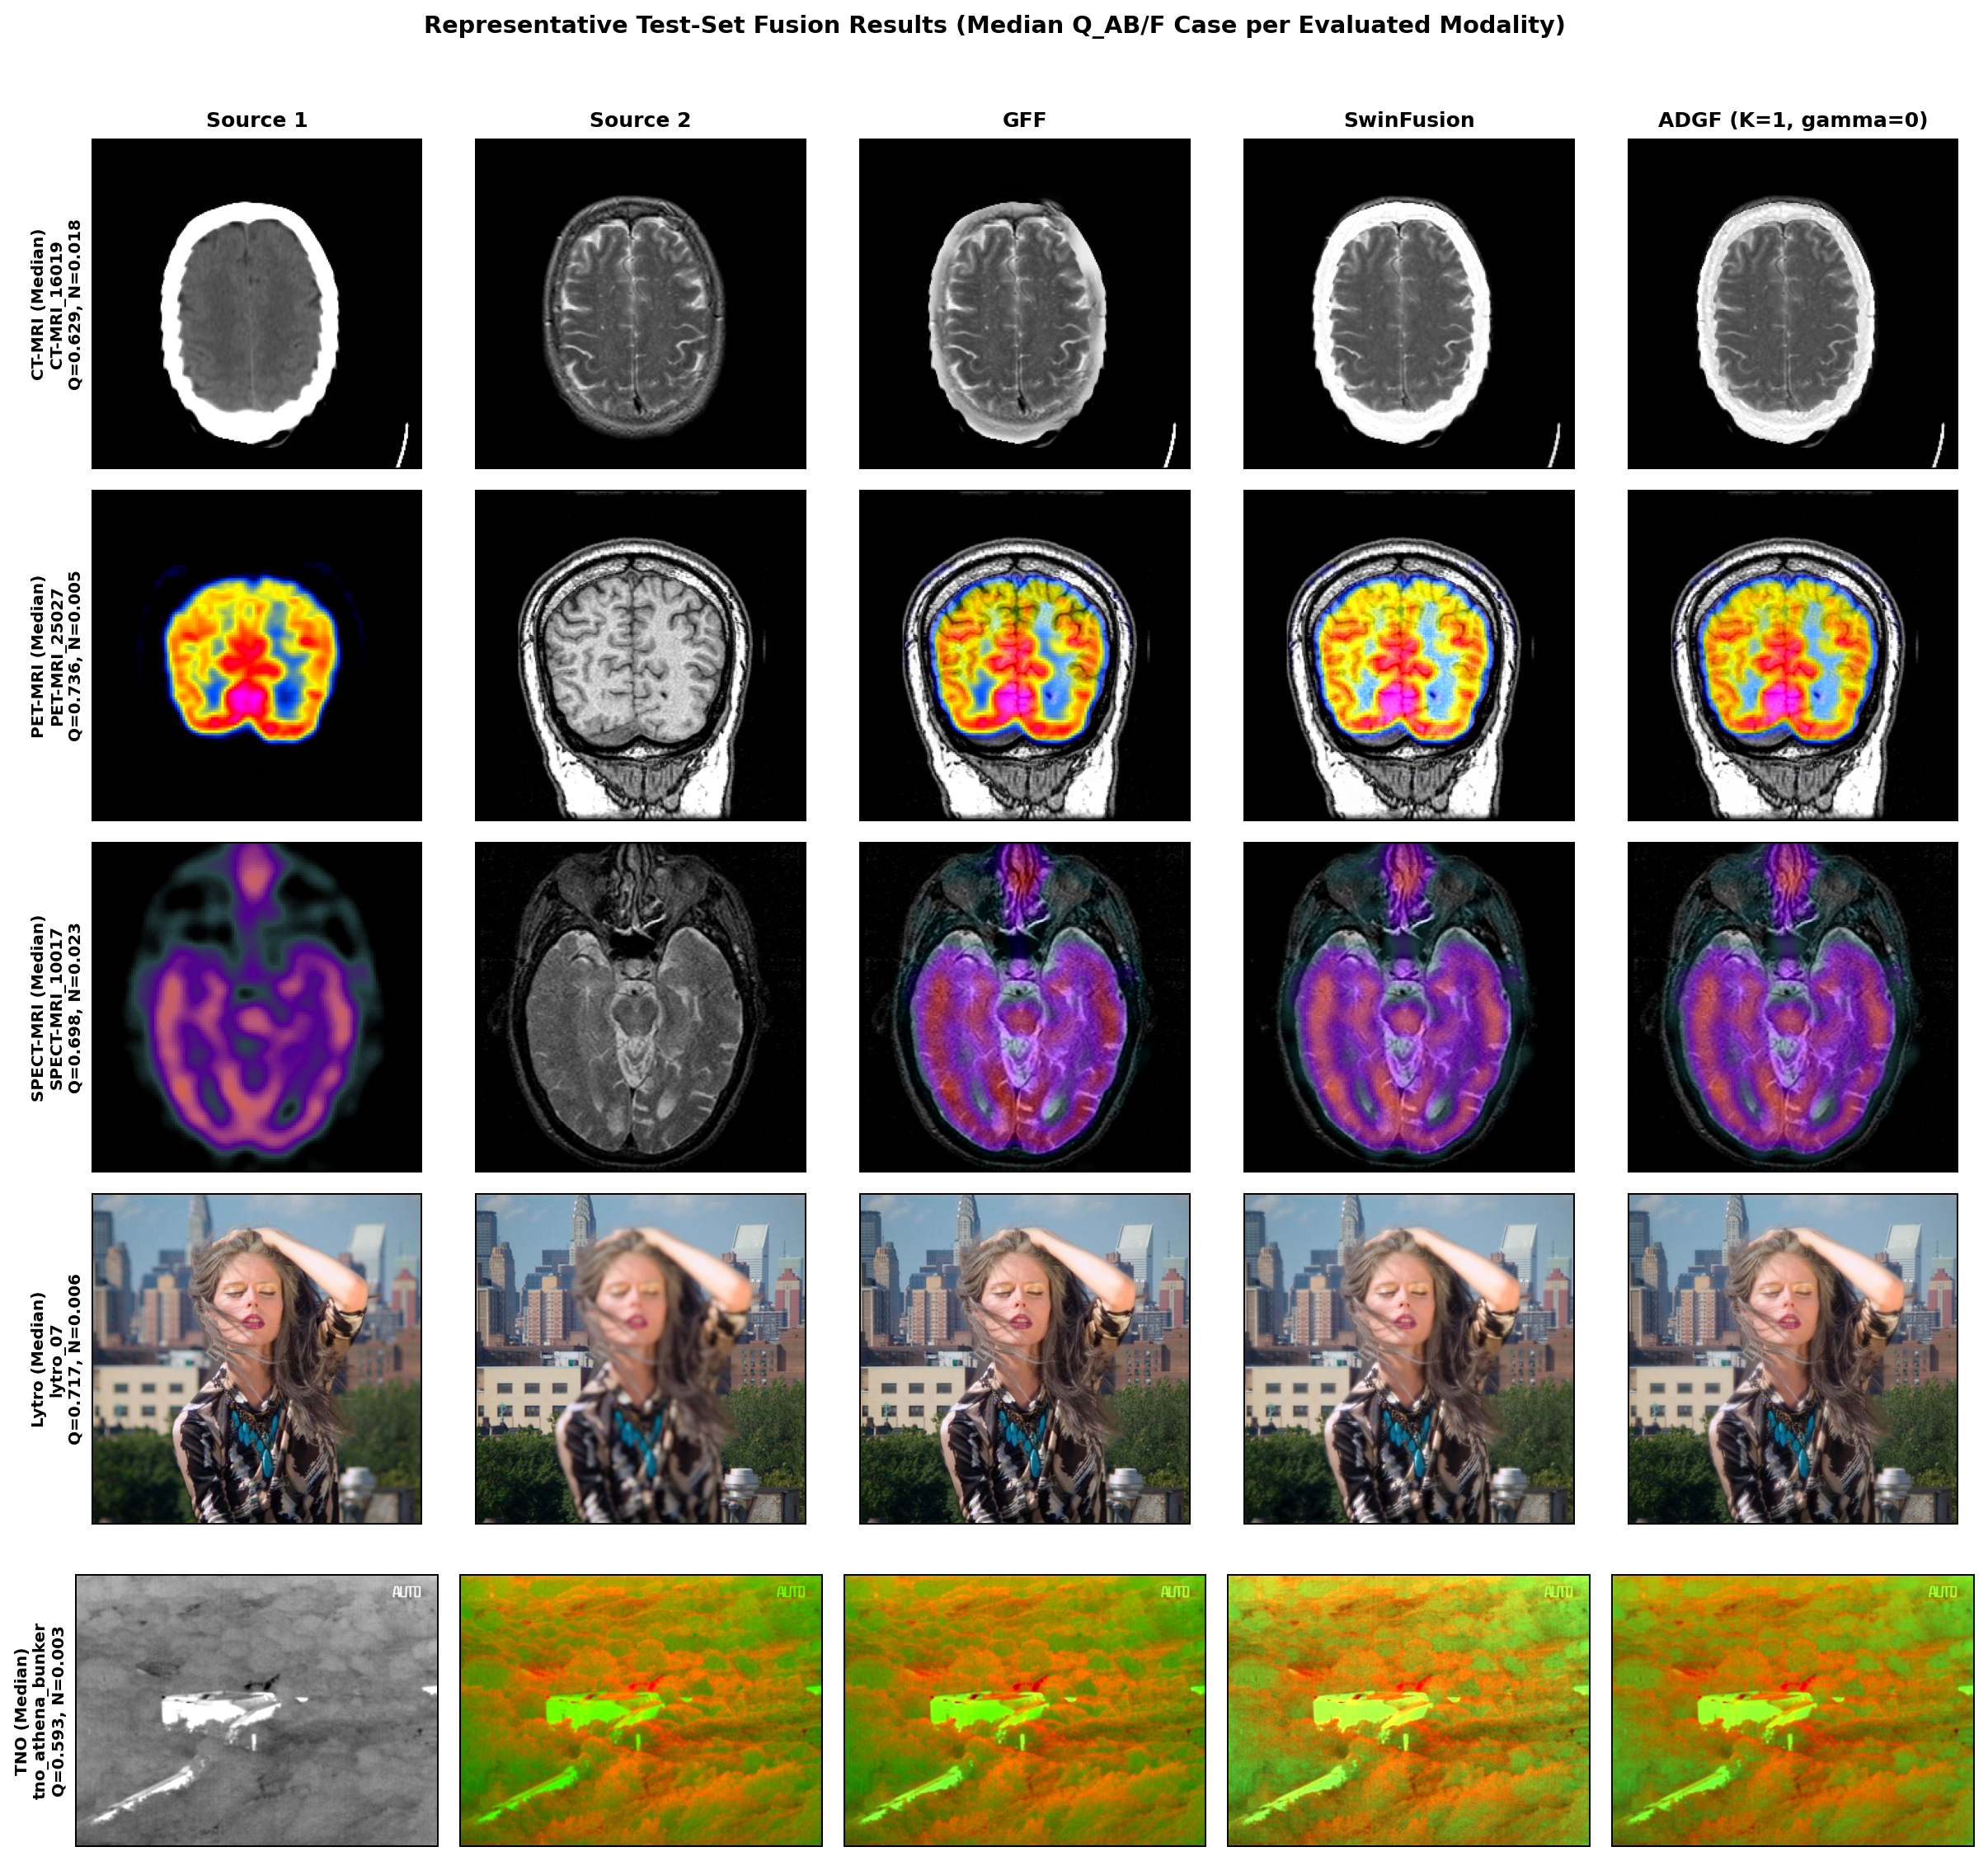
\includegraphics[width=\textwidth]{figures/qualitative_median_cases.png}
\caption{Representative median-$Q^{AB/F}$ test cases across the five evaluated modalities.}
\label{fig:qual_median}
\end{figure*}

\begin{figure*}[htbp]
\centering
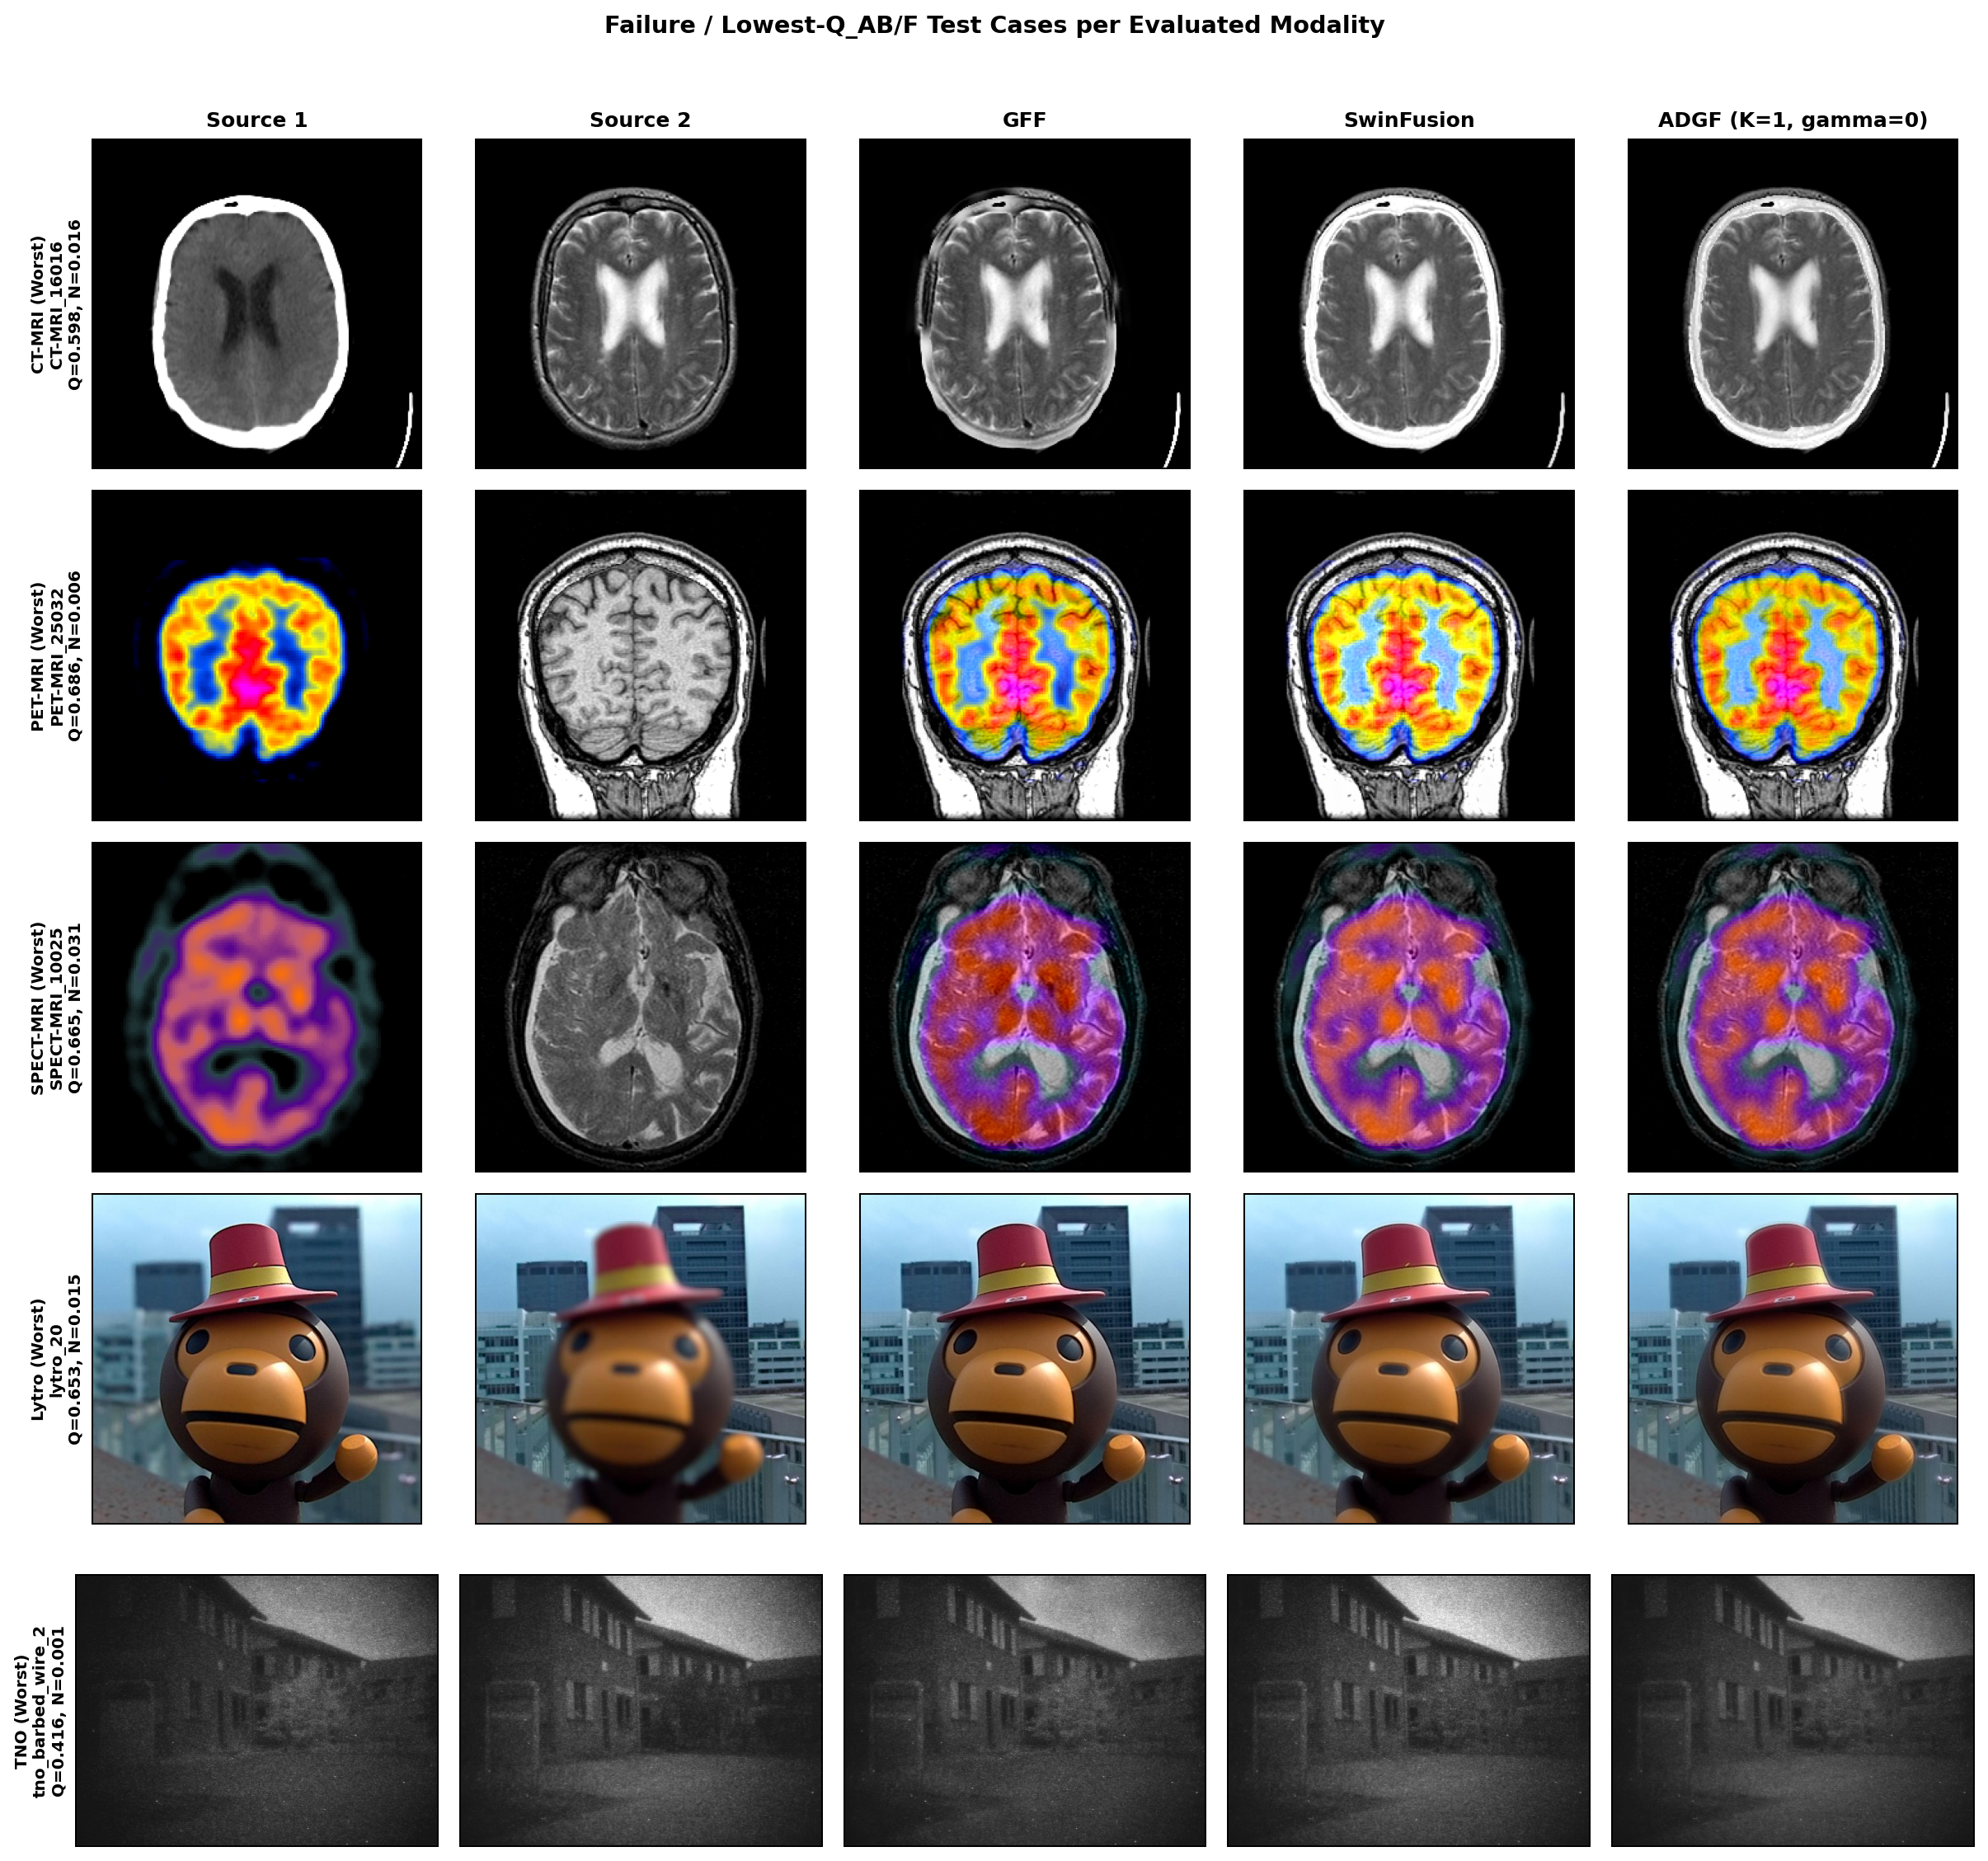
\includegraphics[width=\textwidth]{figures/qualitative_failure_cases.png}
\caption{Lowest-$Q^{AB/F}$ (failure) test cases across the five evaluated modalities.}
\label{fig:qual_failure}
\end{figure*}

\section{Cost and Resources}
Measured on an Intel Core i5-12450H CPU (PyTorch 2.15.0+cpu, \texttt{CUDA: False}), frozen ADGF ($K=1, \gamma=0$) ran in $88.2\pm 35.1\text{ ms}$ on $256\times 256$ CT-MRI (vs GFF $27.4\text{ ms}$, DenseFuse $317.8\text{ ms}$, U2Fusion $627.5\text{ ms}$, SwinFusion $9950.3\text{ ms}$) and $1562.4\pm 264.4\text{ ms}$ on $520\times 520$ Lytro (vs GFF $257.8\text{ ms}$, SwinFusion $53770.5\text{ ms}$). Peak RSS RAM on the five sanity pairs ranged from $115.8$ to $342.3\text{ MB}$ for ADGF prototype vs $111.7$--$342.1\text{ MB}$ for GFF and $250.5$--$638.7\text{ MB}$ for SwinFusion (which ran in 9--45 s when GPU-accelerated on GTX 1650). We make no claim about embedded suitability.

\section{Limitations}
\begin{itemize}
    \item Only 78 of 683 test pairs and 7 of 11 planned methods are populated in \texttt{results/phase4\_test\_metrics.csv}; MSRS (361), RoadScene (220), 24 TNO pairs, and ADF/CBF/SWT/CDDFuse remain pending.
    \item The final configuration is structurally close to GFF and loses to GFF on $Q^{AB/F}$, $\mathrm{VIFP}$, and overall $MI$ while winning on $SSIM$ and lower $N^{AB/F}$.
    \item Hyperparameters were selected one at a time on 120 dev pairs; interactions were not explored.
    \item $N^{AB/F}$ lacks a second independent external Python implementation; no reader study or downstream-task evaluation was performed.
    \item The $\lambda \le 1/4$ stability argument covers the explicit diffusion scheme only; baseline provenance relies on published descriptions.
\end{itemize}

\section{Conclusion}
We presented a training-free diffusion-based fusion pipeline and a pre-registered, leakage-controlled evaluation of it. On 120 development pairs, unclustered global saliency weighting ($K=1$) and removal of additive gradient compensation ($\gamma=0$) achieved the best mean rank ($2.80$ over 14 configurations; $2.40$ over 13), documenting both as negative results relative to our original design. Across the 78 held-out test pairs currently recorded in \texttt{results/phase4\_test\_metrics.csv}, frozen ADGF does not outperform GFF on edge transfer ($Q^{AB/F}$) or $\mathrm{VIFP}$, but delivers significantly lower artifact noise ($N^{AB/F}$) and higher structural similarity ($SSIM$), outperforms DWT and U2Fusion across all primary metrics, and matches or exceeds in-domain SwinFusion on $Q^{AB/F}$, $N^{AB/F}$, $MI$, and $\mathrm{VIFP}$ without GPU requirements or training data. Future work: completing the remaining test datasets and baselines, signed edge-injection schemes, independent $N^{AB/F}$ implementations, downstream-task evaluation, and reader studies.

\section*{Reproducibility}
Code, frozen configuration (\texttt{config.yaml}, \texttt{K\_1\_gamma\_0.0}, seed 42), selection rule (\texttt{selection\_rule.md}), and split lists (\texttt{splits.yaml}, seed 0; exact test pair IDs in \texttt{results/phase4\_test\_metrics.csv}): repository \texttt{Image\_Fusion}, pre-registration commit \texttt{adae0ed3}, code commit \texttt{de03fd9}. Runtime versions: Python 3.12.4, PyTorch 2.15.0+cpu, NumPy 1.26.4, SciPy 1.15.3, OpenCV 4.10.0, scikit-image 0.23.2, scikit-learn 1.4.2, PyWavelets 1.5.0, pandas 2.2.2, \texttt{sewar}.

\begin{thebibliography}{16}
\bibitem{perona1990scale} P. Perona and J. Malik, ``Scale-space and edge detection using anisotropic diffusion,'' \textit{IEEE TPAMI}, vol. 12, no. 7, pp. 629--639, 1990.
\bibitem{he2013guided} K. He, J. Sun, and X. Tang, ``Guided image filtering,'' \textit{IEEE TPAMI}, vol. 35, no. 6, pp. 1397--1409, 2013.
\bibitem{li2013image} S. Li, X. Kang, and J. Hu, ``Image fusion with guided filtering,'' \textit{IEEE TIP}, vol. 22, no. 7, pp. 2864--2875, 2013.
\bibitem{bavirisetti2016two} D. P. Bavirisetti and R. Dhuli, ``Fusion of infrared and visible sensor images based on anisotropic diffusion and Karhunen-Loeve transform,'' \textit{IEEE Sensors J.}, vol. 16, no. 1, pp. 203--209, 2016.
\bibitem{kumar2015image} B. K. S. Kumar, ``Image fusion based on pixel significance using cross bilateral filter,'' \textit{Signal, Image and Video Processing}, vol. 9, no. 5, pp. 1193--1204, 2015.
\bibitem{li2019densefuse} H. Li and X.-J. Wu, ``DenseFuse: A fusion approach to infrared and visible images,'' \textit{IEEE TIP}, vol. 28, no. 5, pp. 2614--2623, 2019.
\bibitem{xu2022u2fusion} H. Xu, J. Ma, J. Jiang, X. Guo, and H. Ling, ``U2Fusion: A unified unsupervised image fusion network,'' \textit{IEEE TPAMI}, vol. 44, no. 1, pp. 502--518, 2022.
\bibitem{zhao2023cddfuse} Z. Zhao et al., ``CDDFuse: Correlation-driven dual-branch feature decomposition for multi-modality image fusion,'' in \textit{Proc. CVPR}, pp. 5906--5916, 2023.
\bibitem{ma2022swinfusion} J. Ma, L. Tang, F. Fan, J. Huang, X. Mei, and Y. Ma, ``SwinFusion: Cross-domain long-range learning for general image fusion via Swin Transformer,'' \textit{IEEE/CAA J. Autom. Sin.}, vol. 9, no. 7, pp. 1200--1217, 2022.
\bibitem{mallat1989theory} S. G. Mallat, ``A theory for multiresolution signal decomposition,'' \textit{IEEE TPAMI}, vol. 11, no. 7, pp. 674--693, 1989; G. P. Nason and B. W. Silverman, in \textit{Wavelets and Statistics}, pp. 281--299, 1995; A. L. da Cunha et al., \textit{IEEE TIP}, vol. 15, no. 10, pp. 3089--3101, 2006.
\bibitem{datasets} L. Tang et al., \textit{Information Fusion}, vol. 83--84, pp. 79--92, 2022 (MSRS); H. Xu et al.~\cite{xu2022u2fusion} (RoadScene); A. Toet, \textit{Data in Brief}, vol. 15, pp. 249--253, 2017 (TNO); K. A. Johnson and J. A. Becker, ``The Whole Brain Atlas,'' Harvard Medical School, 1999; M. Nejati et al., \textit{Information Fusion}, vol. 25, pp. 72--84, 2015 (Lytro).
\bibitem{xydeas2000objective} C. S. Xydeas and V. Petrovic, ``Objective image fusion performance measure,'' \textit{Electronics Letters}, vol. 36, no. 4, pp. 308--309, 2000.
\bibitem{petrovic2005} V. Petrovic and C. Xydeas, ``Objective evaluation of signal-level image fusion performance,'' \textit{Optical Engineering}, vol. 44, no. 8, p. 087004, 2005.
\bibitem{sheikh2006image} H. R. Sheikh and A. C. Bovik, ``Image information and visual quality,'' \textit{IEEE TIP}, vol. 15, no. 2, pp. 430--444, 2006.
\bibitem{han2013viff} Y. Han, Y. Cai, Y. Cao, and X. Xu, ``A new image fusion performance metric based on visual information fidelity,'' \textit{Information Fusion}, vol. 14, no. 2, pp. 127–135, 2013.
\bibitem{wang2004image} Z. Wang, A. C. Bovik, H. R. Sheikh, and E. P. Simoncelli, ``Image quality assessment: from error visibility to structural similarity,'' \textit{IEEE TIP}, vol. 13, no. 4, pp. 600--612, 2004.
\bibitem{ma2019fusiongan} J. Ma et al., ``FusionGAN,'' \textit{Information Fusion}, vol. 48, pp. 11--26, 2019.
\bibitem{zhao2023ddfm} Z. Zhao et al., ``DDFM,'' in \textit{Proc. ICCV}, pp. 8048--8059, 2023.
\bibitem{tang2022piafusion} L. Tang et al., ``PIAFusion,'' \textit{Information Fusion}, vol. 83--84, pp. 79--92, 2022.
\end{thebibliography}

\end{document}
